\section{Supervised Planning with XTREE and BELLTREE}
\begin{figure}[!b]
\small
\centering
\resizebox{1\linewidth}{!}{
\begin{tabular}{|p{\linewidth}|} \hline
\begin{minipage}{\linewidth}
\vspace{0.1cm}
\small
{\bf \fig{xtree}.A: Using XTREE}

Using the training data, construct a decision tree. For each test item, find the {\em current} leaf: take each test instance, run it down to a leaf in the decision tree.  
After that,	find the {\em desired} leaf:
\begin{itemize}[leftmargin=3mm]
\item Starting at {\em current}, ascend the tree levels;
\item Identify {\em sibling} leaves; i.e. leaf clusters that can be reached from level $lvl$ that are not same as {\em current}
\item Find the {\em better} siblings; i.e. those with a {\em score} (\#defects) less than $\gamma=0.5$ times the score of {\em current} branch. 
If none found, then repeat for $lvl += 1$. Also, return no plan if the new $lvl$ is above the root. 
\item  Return the {\em closest} better sibling to the {\em current}.
\end{itemize}
Also, find the {\em delta}; i.e. the set difference between conditions in the decision tree branch to {\em desired} and {\em current}. To find that delta: (1)~for discrete attributes, delta is the value from {\em desired}; (2)~for  numerics, delta is the numeric difference; (3)~for numerics  discretized into ranges, delta is a random number selected from the low and high boundaries of the that range. Finally, return the delta as the plan for improving the test instance.\\
\end{minipage}
\begin{minipage}{\linewidth}
\textbf{\fig{xtree}.B: A sample decision tree.\\}
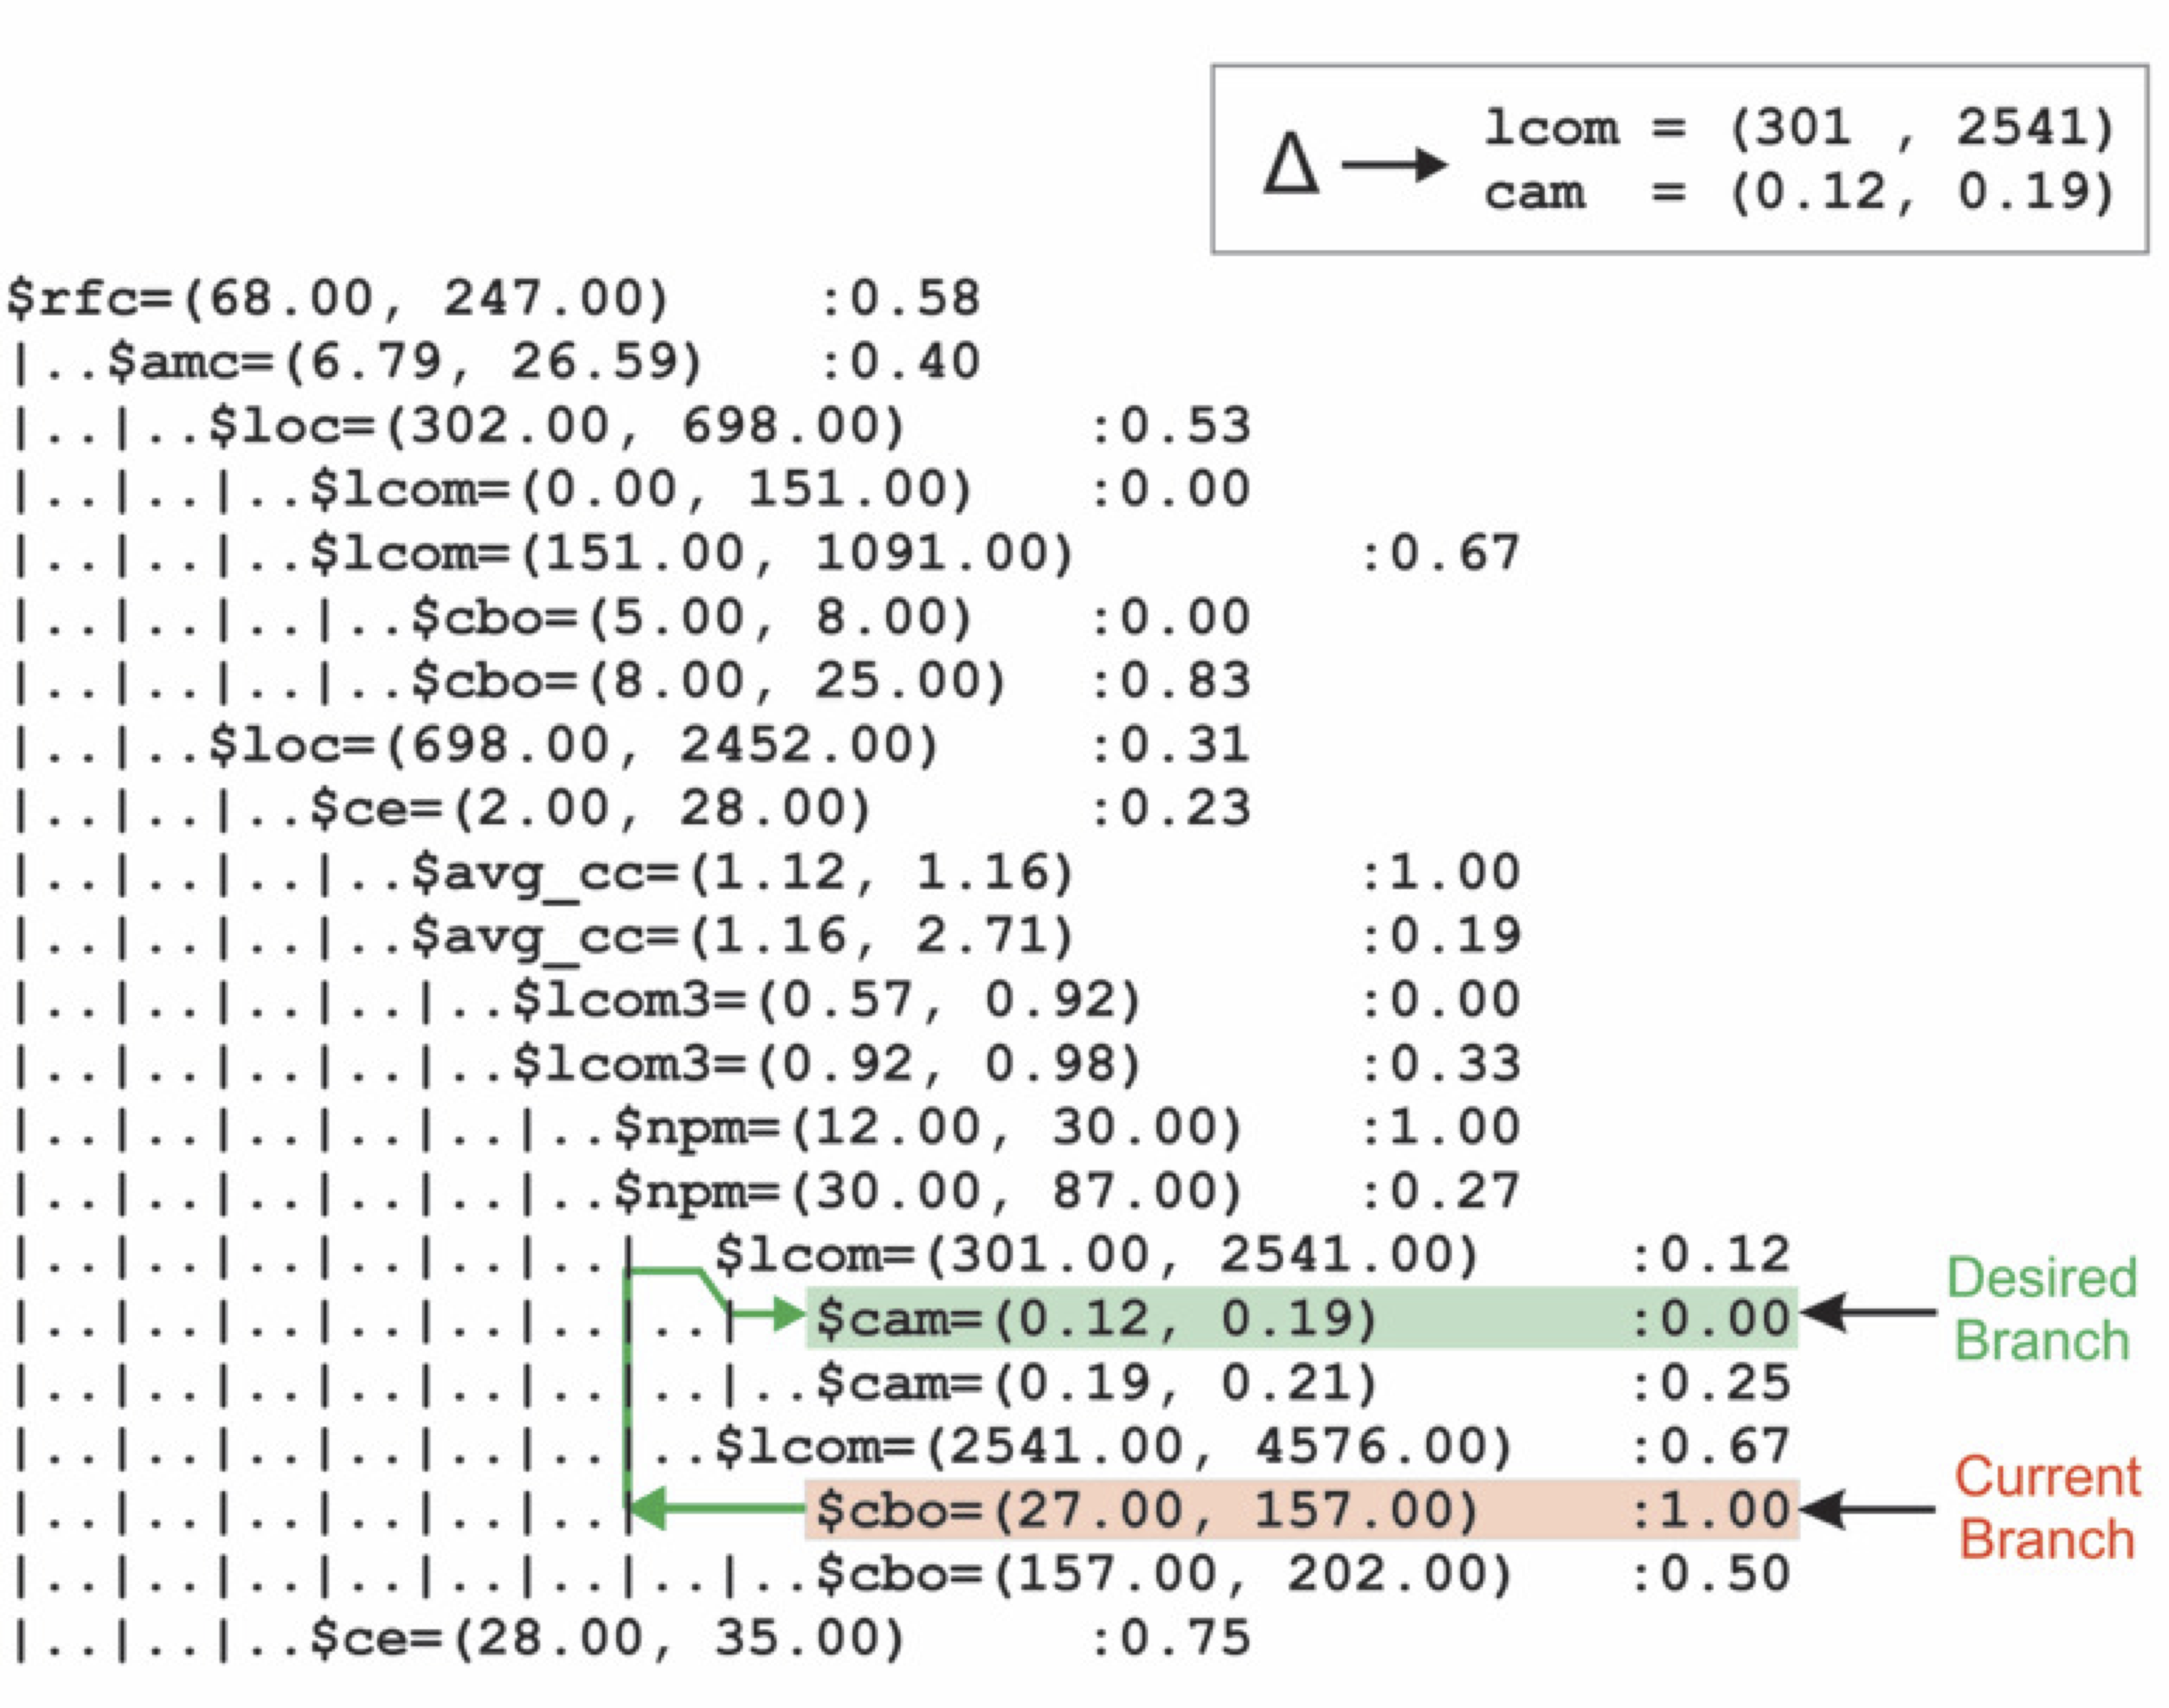
\includegraphics[width=0.99\linewidth]{XTREE_samp.png}
\end{minipage}\bigstrut\vspace{0.1cm}\\\hline
\end{tabular}}
\caption{Generating thresholds using XTREE.}\label{fig:xtree}
\end{figure}
 
 The rest of this paper comparatively evaluates:
 \bi
 \item
The value of the changes proposed
by the above methods (from Alves, Shatnawi,Oliviera et al.);
 \item
Against the changes proposed by the   XTREE/BELLTREE method described below.
\ei

\subsection{\respto{2}\respto{3}Within-Project Planning With XTREE}
\label{sect:XTREE}

Planning with XTREE is comprised of three steps namely, (a)~Frequent pattern mining; (b)~Decision tree construction; and (c)~Planning with random walk traversal. 

\noindent\textbf{Step-1: Frequent pattern mining.} The first step in XTREE is to determine which metrics are most often changed together. The OO metrics tabulated in~\tab{static_metrics} are not independent of each other. In other words, changing one metric (say $\mathit{LOC}$) would lead to a corresponding change in other metrics (such as $\mathit{CBO}$). \respto{3-B} {\color{steel} We refrain from using correlation to determine which metrics change together because correlation measures the existence of a monotonic relationships between two metrics. We cannot assume that the metrics are monotonically related; moreover, it is possible that more than two metrics are related to each other. Therefore, we use frequent pattern mining~\citep{han2007frequent}, which represents a more generalized relationship between metrics, to detect which of the metrics change together.}  

Our instrumentation is shown in~\fig{xtree}.A. We use the FP-Growth algorithm~\citep{han2007frequent} to identify the \textit{maximal frequent itemset} (highlighted in \colorbox{lightgreen}{green} in~\fig{xtree}.A-(d)). This represents the longest set of metrics that change together atleast $\mathit{support}\%$~(in our case $60\%$) of the time. The following steps use the \textit{maximal frequent itemset} to guide the generation of plans.  

\noindent\textbf{Step-2: Decision tree construction.} Having discovered which metrics change together, we next establish what range of values for each metrics point to a high likelihood of defects. For this we use a decision tree algorithm (see~\fig{xtree}.B). Specifically, we do the following: 
\be[wide=0pt]
\item Each of the OO metrics (from~\tab{static_metrics}) are discretized into a range of values with the help of Fayyad-Irani discretizer~\citep{fi}.
\item We sort the OO metrics from the most discriminative  to the least discriminative.
\item We begin by constructing a tree with the most discriminative OO metric, e.g., in~\fig{xtree}.B (b) this would be $\mathit{rfc}$.
\item Then, we repeat the above to steps on the remaing OO metrics. 
\item \respto{2-D} {\color{steel} When we reach a predetermined termination criteria of having \textit{less than $\sqrt{N}$ samples in subsequent splits}, we do not recurse futher. Here, $N$ is the number of OO metrics, i.e., $N=20$.}
\item Finally, we return the constructed decision tree.  
\ee
\respto{2-C} {\color{steel} The leaf nodes of the decision tree contain instances of the training data that are most alike. The mean defect count of these instances represents the defect probability. In the case of~\fig{xtree}.B (b), if $\mathit{rfc}=[0,1),~\mathit{KLOC}=[3,5),~\text{and}~\mathit{DIT}=[1,6)$ then the probability of defect is $0.9$}. 

\noindent\textbf{Step-3: Random Walk Traversal.} With the last two steps, we now know (1) which metrics change together and (2) what ranges of metrics indicate a high likelihood of defects. with this information, XTREE builds plans from the branches of the tree as follows. Given a ``defective'' test instance, we ask:
\be
\item
Which \underline{\textit{current}} node does the test instance fall into?
\item What are all the \underline{\textit{desired}} nodes the test case would want to emulate? These would be nodes with the \textit{lowest} defect probabilities.
\ee

Finally, we implement a random-walk~\citep{ying2018graph, sharma2016graphjet} model to find paths that lead from the \textit{current} node the \textit{desired} node. Of all the paths that lead from the \textit{current} node to the \textit{desired} node, we select the path that has the highest overlap with the \textit{maximal frequent itemset}. As an example, consider~\fig{xtree}.C. Here, of the two possible paths~\fig{xtree}.C(a) and~\fig{xtree}.C(b), we choose that latter because it traverses through all the metrics in the maximal frequent itemset.

{\color{steel}
\subsubsection*{\respto{3-C} How are plans generated?}

The path taken by the random-walk is used to generate a plan. For example, in the case of~\fig{xtree}.C, it works as follows:
\be
\item The test case finds itself on the far left, i.e., the ``current node'' has: $RFC: [0, 1)$, $KLOC: [3,5)$ and $DIT: [1,6)$
\item After implementing the random walk, we find that ``desired'' node is on the far right (highlighed in \colorbox{black}{{\color{white} black}})
\item The path taken to get from the ``current node'' to the ``desired node'' would require that the following changes be made.
\bi
\item[$\circ$] $~RFC:  [0, 1) \longrightarrow [1, 5)$;
\item[$\circ$] $KLOC:  [0, 1) \longrightarrow [1, 3)$; and
\item[$\circ$] $~CBO:  [6, 10)$
\ei
The plan would then be these ranges of values.
\ee
}


\subsection{Cross-project Planning with BELLTREE}
\label{sect:CPXTREE}

Many methods have been proposed for transferring data or lessons
learned from one project to another, for examples see~\citep{Nam2013, Nam2015, jing15, kocaguneli2011find, kocaguneli2012, turhan09, peters15}. Of all these, the bellwether method described here is one of the simplest.
Transfer learning with bellwethers is just a matter of calling existing
learners inside a for-loop. For all the training data from different projects $\mathcal{P, Q, R, S...}$, 
a bellwether learner conducts a round-robin experiment where a model is learned from project, then applied to all others. The {\em bellwether} is that project which generates the best performing model. The {\em bellwether effect}, states that models
learned from this bellwether performs as well as, or better than, other transfer learning algorithms. 

For the purposes of prediction, we have shown previously that bellwethers are remarkably
effective for many different kinds of SE tasks such as (i)~defect prediction, (ii)~effort
estimation, and (iii)~detecting code smells~\citep{krishna17b}. This paper is the first to check the value of bellwethers for the purposes of planning. Note also that this paper's use of bellwethers enables us to generate plans from different data sets from across different projects. This represents a novel and significant extension to our previous work~\citep{krishna17a} which was limited to the use of datasets from within a few projects.



BELLTREE extends the three bellwether operators defined in our previous work~\citep{krishna17b} on bellwethers: DISCOVER, PLAN, VALIDATE. That is:~ 
\be
  \item DISCOVER: {\em Check if a community has bellwether.} 
  This step is similar to our previous technique used to discover bellwethers~\citep{krishna16}. We see if standard data miners can predict for the number of defects, given the static code attributes. This is done as follows:~ 
  \bi 
  \item
  For a community $C$ obtain all pairs of data from
  projects $\mathcal{P, Q, R, S...}$ such that $x, y \in C$;
  \item
  Predict for defects in $y$ using a quality predictor learned from data taken from $x$;
  \item
  Report a bellwether if one $x$ generates consistently high predictions in a majority of $y \in C$.
  \ei
  \respto{2-B} {\color{steel} Note, since the above steps perform an all-pairs comparison, the theoritical complexity of the DISCOVER phase will be be $O(N^2)$ where $N$ is the number of projects.}
  \item PLAN: {\em Using the bellwether, we generate plans that can improve a new project.} That is, 
  having learned the bellwether on past data, we now construct a decision tree similar to within-project XTREE. We then use the same methodology to generate the plans.
  \item VALIDATE: {\em Go back to step 1} if the performance statistics seen during PLAN fail to generate useful actions.
  \ee
  

